\documentclass[10pt,twocolumn]{article}
\usepackage{times}
\usepackage{url}

% do not change these values
\baselineskip 12pt
\textheight 9in
\textwidth 6.5in
\oddsidemargin 0in
\topmargin 0in
\headheight 0in
\headsep 0in

\usepackage{graphicx}
\usepackage{subcaption}
\usepackage{color}
\usepackage{float}
\usepackage{amsmath}
\usepackage{algorithm}
% \usepackage{algorithmic}
\usepackage[noend]{algpseudocode}

\begin{document}

\title{Title}
\author{Zhouwang Fu$^1$ and Zhengwei Qi$^1$ \\
% \small {\em  $^1$Shanghai Jiao Tong University \quad
%           $^2$Cloud National Labs} \\ [2mm]
\small {\em  $^1$Shanghai Jiao Tong University} \\ [2mm]
% \small Submission Type: Research
}
\date{}
\maketitle

\begin{abstract}

Shuffle is the term used to describe the cross-network read and aggregation of partitioned ancestor data before invoking reduce operation.
As DAG computing frameworks keep evolving, calculation and scheduling of each task are well optimized. 
However shuffle cuts off the data processing pipeline, introduce significant latency to successors.
To remove shuffle overhead, we present SCache, a plugin system to decouple shuffle from DAG computing framework. SCache captures shuffle data in the memory and uses heuristic-MinHeap scheduling to balance data blocks to eliminate the explicit barrier. We implement SCache and change Spark to use SCache as external shuffle service and co-scheduler. We evaluate SCache performance both on simulation and 50-machines Amazon EC2 cluster.
Results show that, by incorporating SCache, the shuffle overhead of Spark can be reduced in overall 90\%.

\end{abstract}

\section{Introduction}

\section{Motivation}

In this section, we first study the shuffle pattern (\ref{shuffle pattern}) . 
Then we show the observations of the opportunities to optimize shuffle in \ref{observation}
\subsection{Characteristic of Shuffle} \label{shuffle pattern}

In large scale data parallel computing, enormous datasets are partitioned into pieces to fit the memory of each node since the very beginnig of MapReduce\cite{mapreduce}.
Meanwhile, complicated application procedures are divided into steps. The successor steps take the output of ancestors as input to do the computation. Shuffle occurs when each successor needs 
part of data from all ancestors' output. In order to provide a clear illustration, we define those computing each partition of data in one step as task. For tasks that generates shuffle output, we call
them map task. For tasks that consume shuffle output, we call them reudce tasks. Note that one task may have both shuffle data generation and consumption in mordern DAG framework. These tasks contains characteristic of both map task and reduce task. But these tasks won't change the behavior of shuffle. To avoid ambiguity, in the following paper, we will only use term of map task to represent those who produce shuffle output, and reduce task to represent those who consume shuffle output.

Shuffle is designed to achieve an all-to-all data blocks transfer among nodes in cluster. It exists in both MapReduce models and DAG computation models.

The overview process of shuffle is presented in Firgure \ref{fig:shuffle_process}. Shuffle mainly contains two phases itself: \textbf{Data Partition} and \textbf{Data Transfer}. For \textbf{Data Partition}, each map task will partition the result data (key, value pair) into several buckets according to the partition function.
The buckets number equals to the number of tasks in the next step. When the map tasks finish, all the shuffle output data will be written into local persistent storage for fault tolerance \cite{mapreduce, spark}.
\textbf{Data Transfer} can be further divied into two parts: \textbf{Shuffle Write} and \textbf{Shuffle Read}. \textbf{Shuffle Write} starts after execution of map tasks and intermediate tasks. Partitioned data will  be stored on disk during \textbf{Shuffle Write}. \textbf{Shuffle Read} starts at the beginning of reduce tasks tasks. These tasks will fetch the data that belongs to their corresponding partitions from both remote nodes and local storage.

In short, shuffle is loosely coupled with application context and it's I/O intensive.

Since intensive I/O operation will be triggered during a shuffle, this can introduce a significant lantency to the application. Reports show that, 60\% of MapReduce jobs at Yahoo
and 20\% at Facebook are shuffle intensive workloads\cite{shufflewatcher}. For those shuffle intensive jobs, the shuffle lantency may even dominate Job Completion Time. 
For instance, a MapReduce trace analysis from Facebook shows that shuffle accounts for 33\% JCT on average, up to 70\% in shuffle intensive jobs\cite{managing}.
Meanwhile, the completion time of shuffle correlates with the performance of storage devices, network and even applications. 
This variation may bring a huge challenge for operators to find the correct configuration of the DAG framework.
\begin{figure}
	\centering
	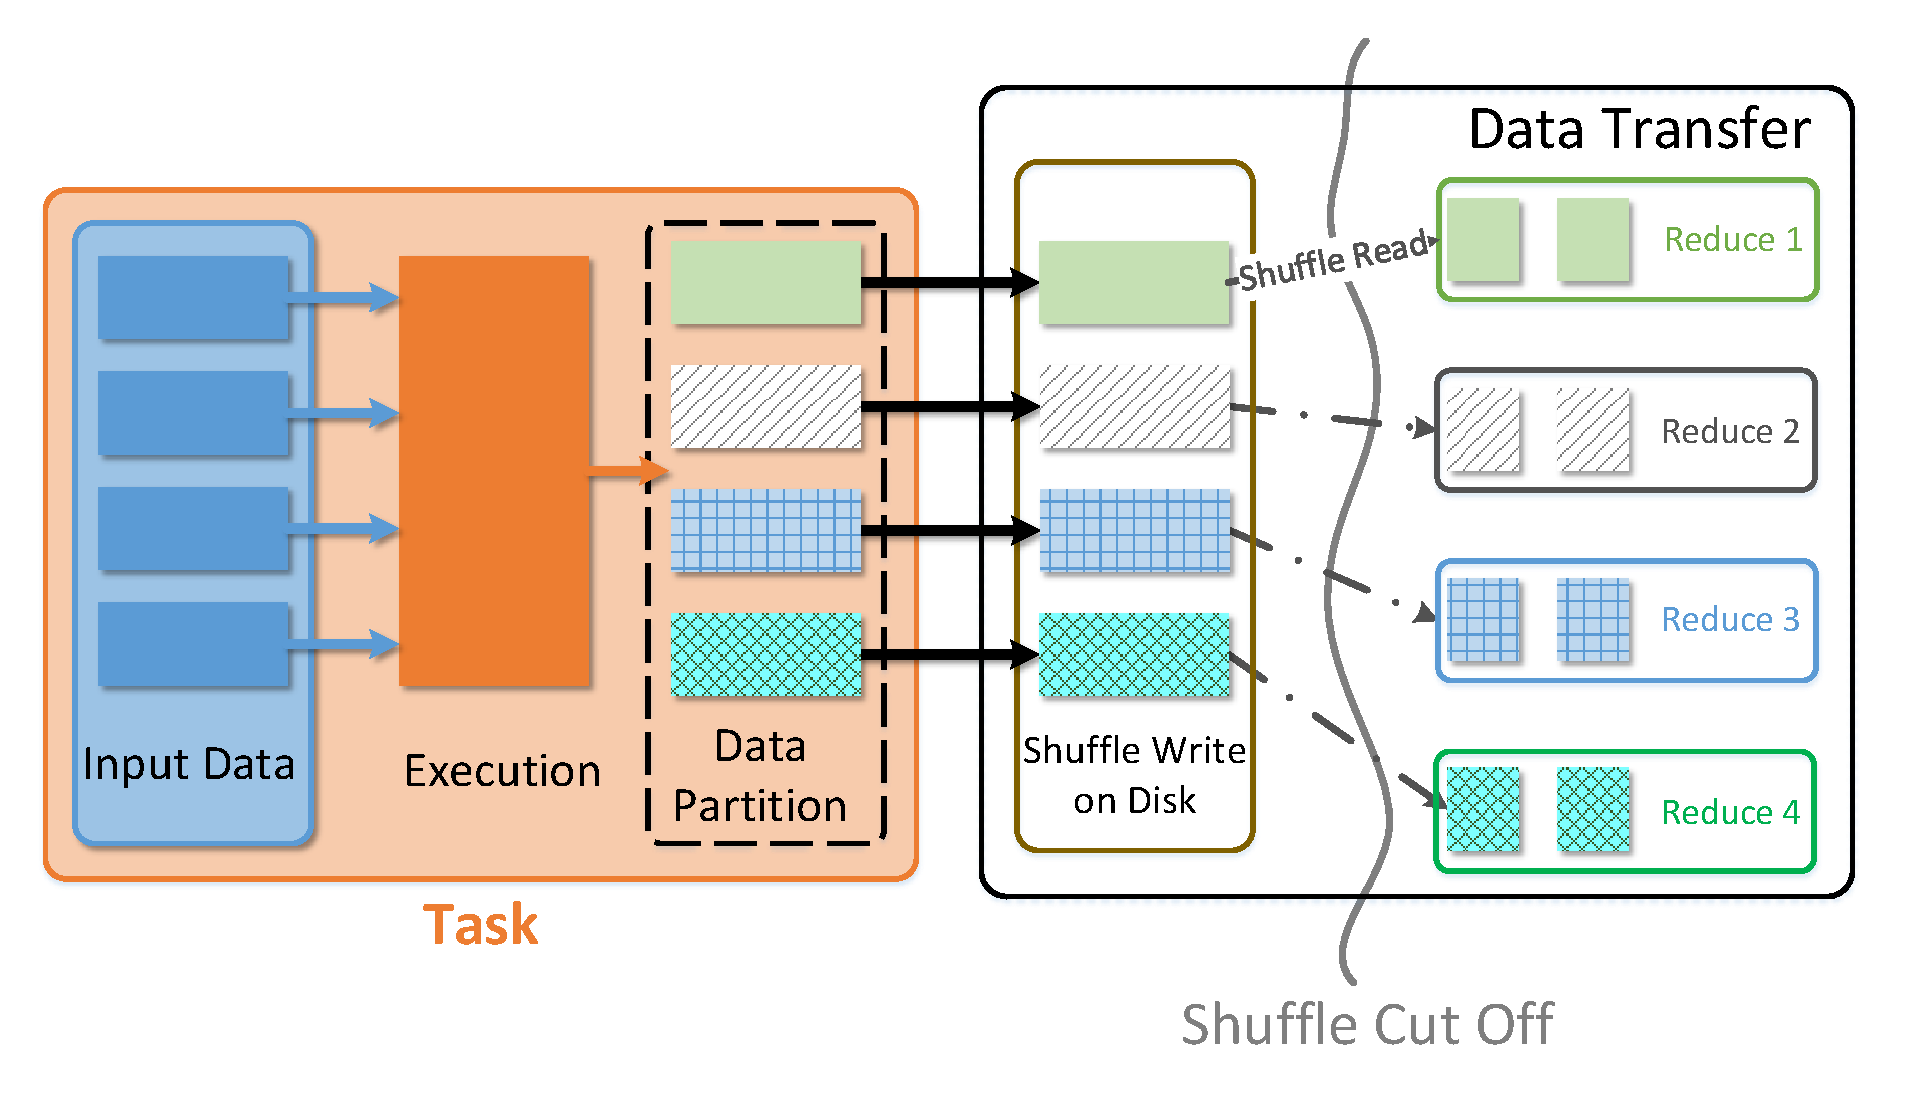
\includegraphics[width=\linewidth]{fig/shuffle_process}
	\caption{Shuffle Overview}
	\label{fig:shuffle_process}
\end{figure}

\subsection{Observations} \label{observation}
Of course, shuffle is unavoidable in a DAG computing process. But \textit{can we mitigate or even remove the overhead of shuffle?} To find the answers, we run some representative applications on a Spark in a 5 m4.xlarge Aamzon EC2 cluster. We than capture and plot the CPU utilization, I/O throughput and tasks execution information on each node. Take the trace in Figure \ref{fig:util} as an example, which is caputured during one Spark GroupByTest job. This job has 2 rounds of tasks for each node. We mark the 'Execution' phase in the figure from the launch time of the first task on this node to the execution finish timestamp of the last one. The 'Shuffle Write' phase is marked from the timestamp of the begining of the first partitioned data write. The 'Shuffle Read and Execution' phase is mark from the start of the first reduce launch timestamp.
Figure \ref{fig:util} contains data including two stages connected by one shuffle. By analyzing the trace combing with Spark, we propose following observations.
\begin{figure*}
	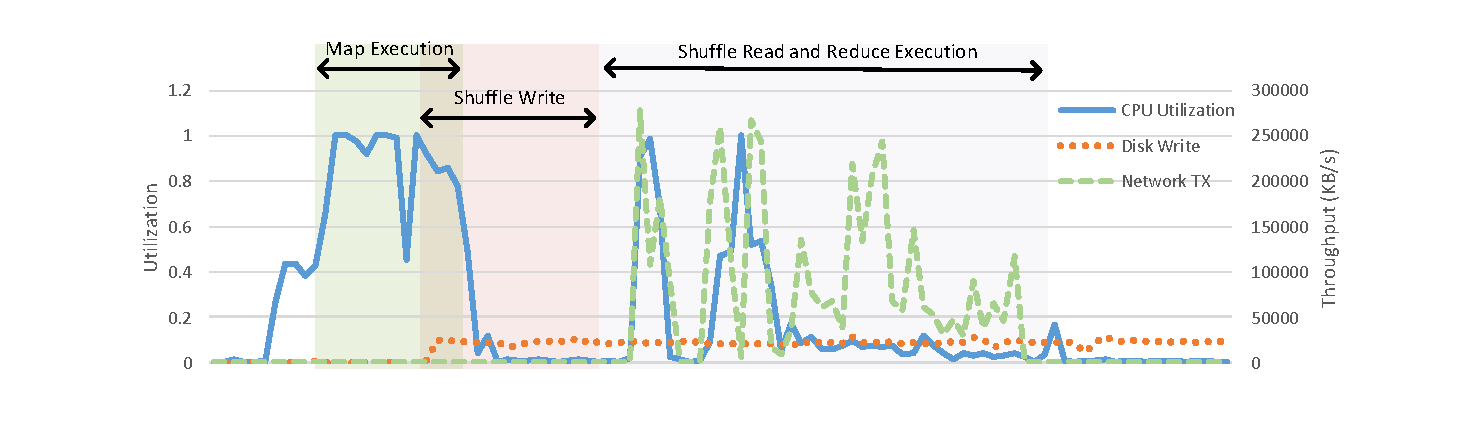
\includegraphics[width=\textwidth]{fig/util}
	\caption{CPU utiliazation and I/O throughput of a node during a Spark single shuffle application}
	\label{fig:util}
\end{figure*}

\subsubsection{Multi-rounds tasks in each stages}\label{multi}
Both experiece and DAG framework manuals recommand that multi-rounds execution of each stage will benifit the performance of whole application.
For example, Hadoop MapReduce Tutorial \cite{hadooptutorial} suggests that \textit{10-100 maps per-node} and \textit{0.95 or 1.75 $\times$ no. of nodes $\times$ no. of maximum container per node} seem to be the right level of parallelism. Spark Configuration also recommends 2-3 tasks per CPU core in the cluster\cite{sparkconf}.
We have two rounds of tasks in job of Figure \ref{fig:util} to process about 70GB data. Figure \ref{fig:util} shows that the second phase of shuffle -- \textbf{Data Transfer} will start until the reduce stage starts.
But the shuffle data will become available as soon as the execution of one task is finished. Though in the context of Spark, the reduce task can do compuation while fetching data, the uncontrolled network congestion may still hurt the performance. However, if the destination of the shuffle output of each task is aware, the property of mutil-round can be leveraged to do \textbf{Data Transfer} ahead of reduce stage.

\subsubsection{Tight copule between shuffle and computation}
Another information we get from the trace is that shffle should be decoupled from task which is a execution unit in both Spark and Hadoop MapReduce. In general, CPU and memory are binded as a schedule slot in DAG resource scheduler. When a task is scheduled to a slot, it won't release until it reaches the end of task. In Figure \ref{fig:util}, the resource of Spark executor will be realsed at the ending of 'Shffle Write'.
But CPU becomes idle almost as soon as the 'Exectuion' is finished. On the other hand, shuffle is I/O intensive job. It doesn't involved CPU and application context. If the shffle can be decopled from task, the slot can be relased after 'Execution' phase. The early release can benifit other tasks to achieve better overall performance of the DAG framework.

\subsubsection{I/O performance varys}
When we look into the performance of disk and network in our test case, there is huge variance. Since we use the standard EBS as our backend storage for the EC2 instances, the I/O performance of disk is poor. 
At the same time, the exclusive bandwidth of each instance is 750 Mbps\cite{aws}. In this case, the bottleneck of shuffle is disk, which introduces a significant latency for the application. Vice versa, in some cases, the congestion of network may also become the bolltle of shuffle\cite{varys}. The uncertainty of the I/O performance cause a huge challenge for optmizing the DAG computing in the cluster. For network latency, the most we can do is to mitigate the transfer delay. As for disk write, we believe it's not necessary for today's cluster. Recall that the persistence of shuffle data is used only for reduce fault tolerence, but mean time to failure(MTTF) for a server is counted in the scale of year\cite{tachyon}. In addition, we believe combing the high speed of network and memory is a better choice for fault tolerence. We will present more details in Section \ref{impl}.

\subsubsection{Shuffle size is small}\label{shufflesize}
In order to accelearte computation, Spark will put all the input data set for a task into memroy. Comparing to the input dataset, size of shuffle data is relatively small. We persent to typical application on Spark to show the releationship between shuffle data comparing with the input dataset in Figure \ref{fig:shuffle_size}. Although TeraSort\cite{terasort} is known as a shuffle intensive job, in a 10GB input TeraSort, the shuffle size is less than 3GB. When it's mapped to a 5 nodes cluster, it only taks about 500MB memory (\~25\% of input size for each node) to cache the shuffle data in memory. The data reported in \cite{makingsense} also shows that the amount of data shuffled is less than input data, by as much as a factor of 5-10. This is another reason that disk should not be involved in the whole shuffle procedure.


Based on these observations, it's straightforward to come up with a optimization to use memory to store the shuffle data and overlap the I/O operations of shuffle
by leveraging multi-rounds property of DAG computing. In order to achieve this optimization, we have to decouple shuffle from task and 
perform pre-fetch as soon as each output of map task and intermediate task is available. But is this feasible? We try to answer this question
in the following sections.

\section{Achieve Shuffle Optimization}
In this section, we try to achieve shuffle optimization by applying
\begin{itemize}
	\item Decouple shuffle from task
	\item Pre-fetch shuffle to reduce node
\end{itemize}
on the DAG computing framwork.
We choose Spark as the representative of DAG computing framwork to implement our optimization.
\subsection{Decouple shuffle from task}
On the map task side of shuffle, it's used to partition the output of map task according to the pre-defined partitioner. More specifically, shuffle takes a set of key-value pairs as input. And than it calculates the partitioner number of a key-value pait by applying pre-defined the partition function to the key. At last it put the key-value pair into the coressponding parition. The output at last is a set of blocks. Each of them contains the key-value pairs for one partition. For those application context unrelated blocks, they can be easily hijacked in the memory of Spark executor and moved out of JVM space via memory mapping. Meanwhile, we have to prevent the memory spill during the shuffle partition procedure, so that the shuffle data can never touch the disk. The default shuffle spill threshold in Spark is 5GB\cite{sparksource}, which is big enough in most scenarios according to Section \ref{shufflesize}.

\subsection{Pre-schedule with Application Context}
When the shuffle output blocks are available in memory, they can be pre-fetched to the remote hosts to hide the network transfer time. But at that time, the reduce tasks taking shuffle as input are still pending. In other word, the remote hosts of those blocks keep unknown until the reduce tasks are scheduled by the DAG framework. In order to break this serialization between map tasks and shuffle, we have to first pre-schedule the task-node mapping ahead of DAG framework scheduler. We explore several pre-scheduling schemes in different scenrios. And evalute the performance of pre-scheduling and prediction by calculating the improvment of reduce tasks completion time with trace of OpenCloud\cite{opencloudtrace}. We first emulate the sheduling algorithm of Spark to schedule the reduce tasks of one job, and take the bottleneck of the task set as the completion time. Then we remove the shuffle read time as the assumption of shffle data pre-fetch and emulate under different schemes. The result is shown in \ref{fig:sim}.
\begin{figure*}
	\centering
	\begin{minipage}{0.34\linewidth}
		\begin{figure}[H]
			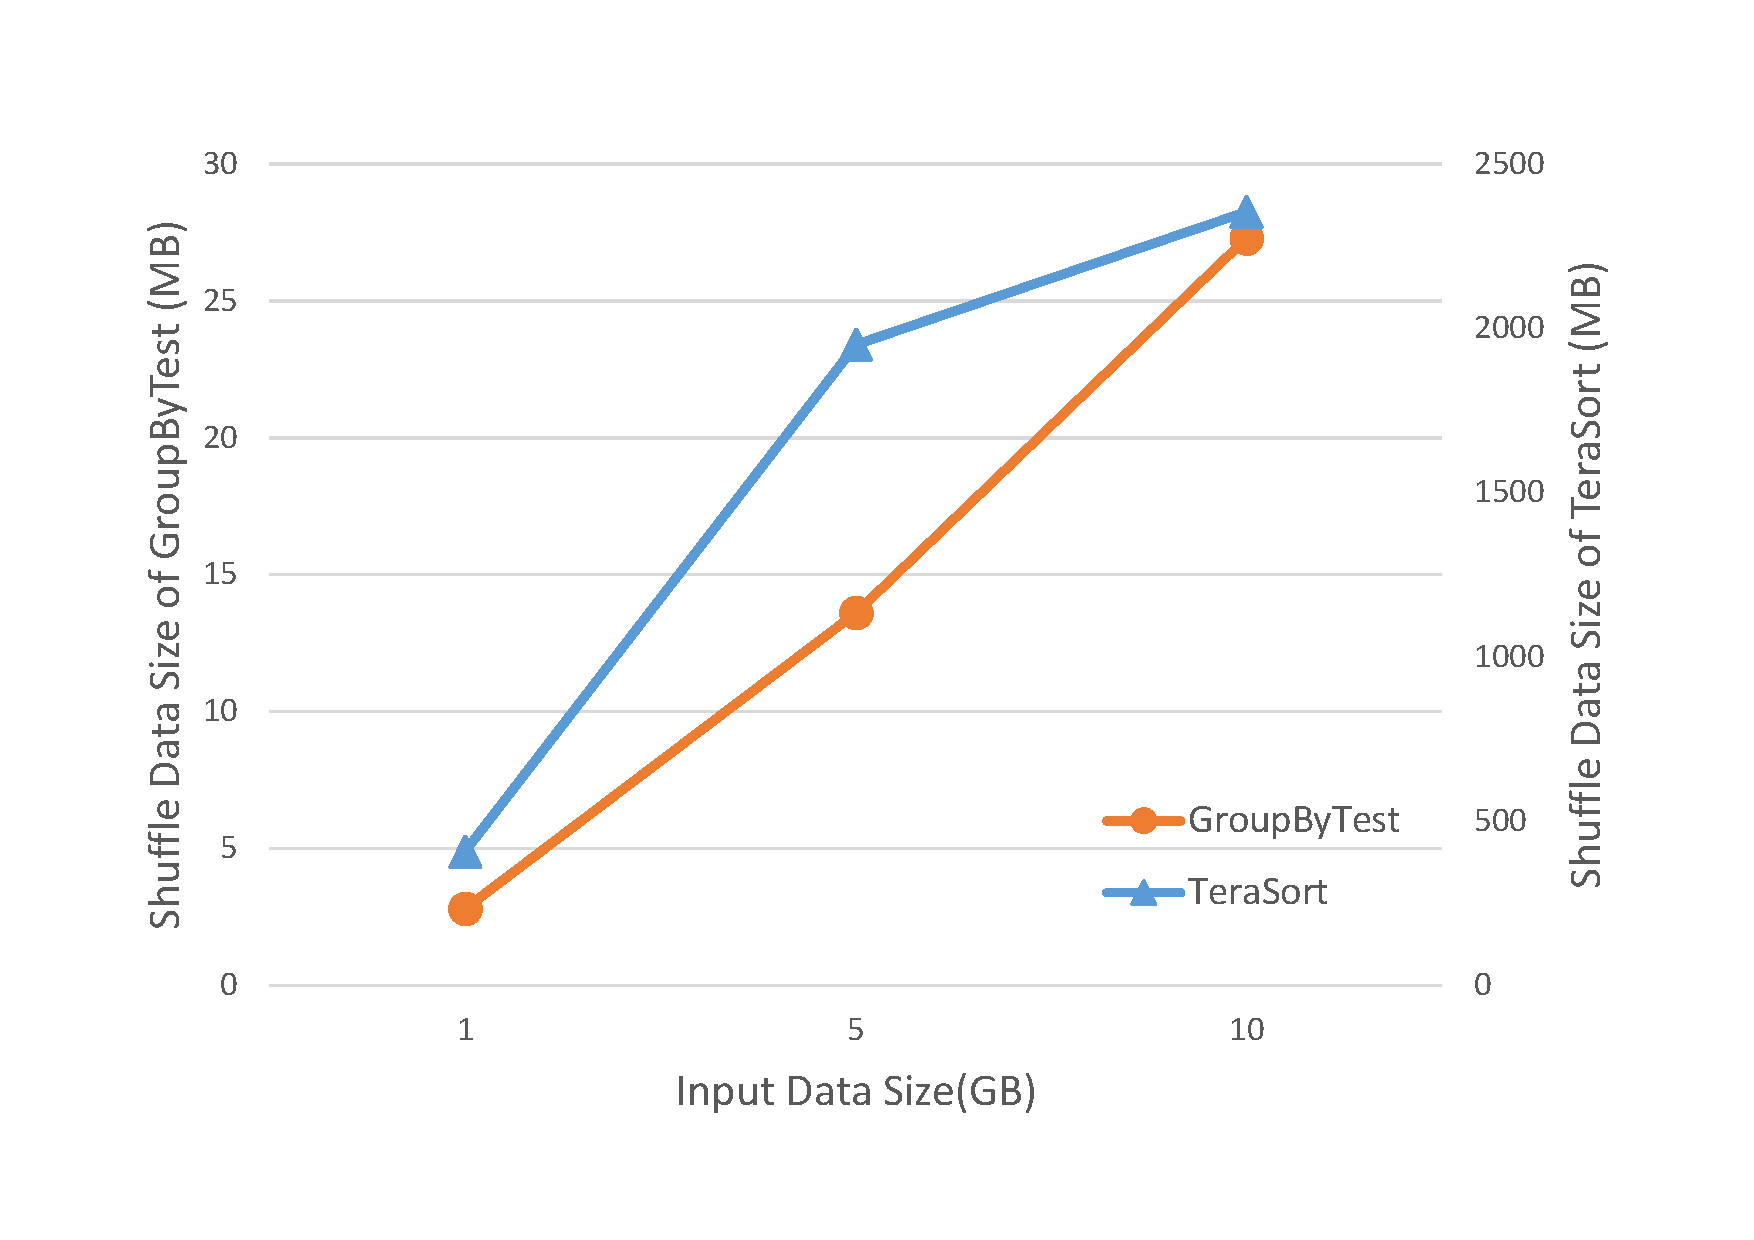
\includegraphics[width=\textwidth]{fig/shuffle_size}
			\caption{Shuffle Size Comparing with Input Size}
			\label{fig:shuffle_size}
		\end{figure}
	\end{minipage}
	\begin{minipage}{0.65\linewidth}
		\begin{figure}[H]
			\begin{subfigure}{0.5\textwidth}
				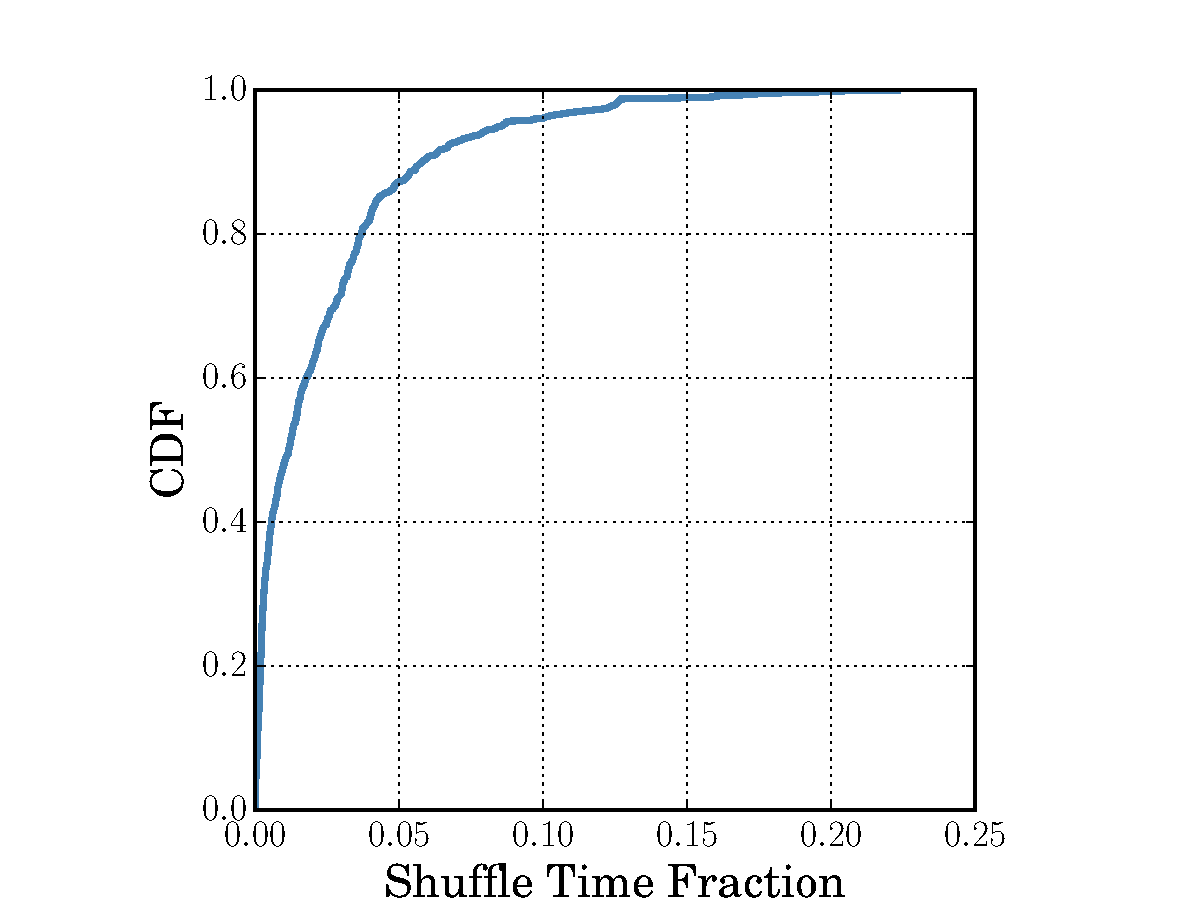
\includegraphics[width=\linewidth]{fig/reduce_cdf}
				\caption{Shuffle Time Fraction CDF}
				\label{fig:cdf}
			\end{subfigure}	
			\begin{subfigure}{0.5\textwidth}
				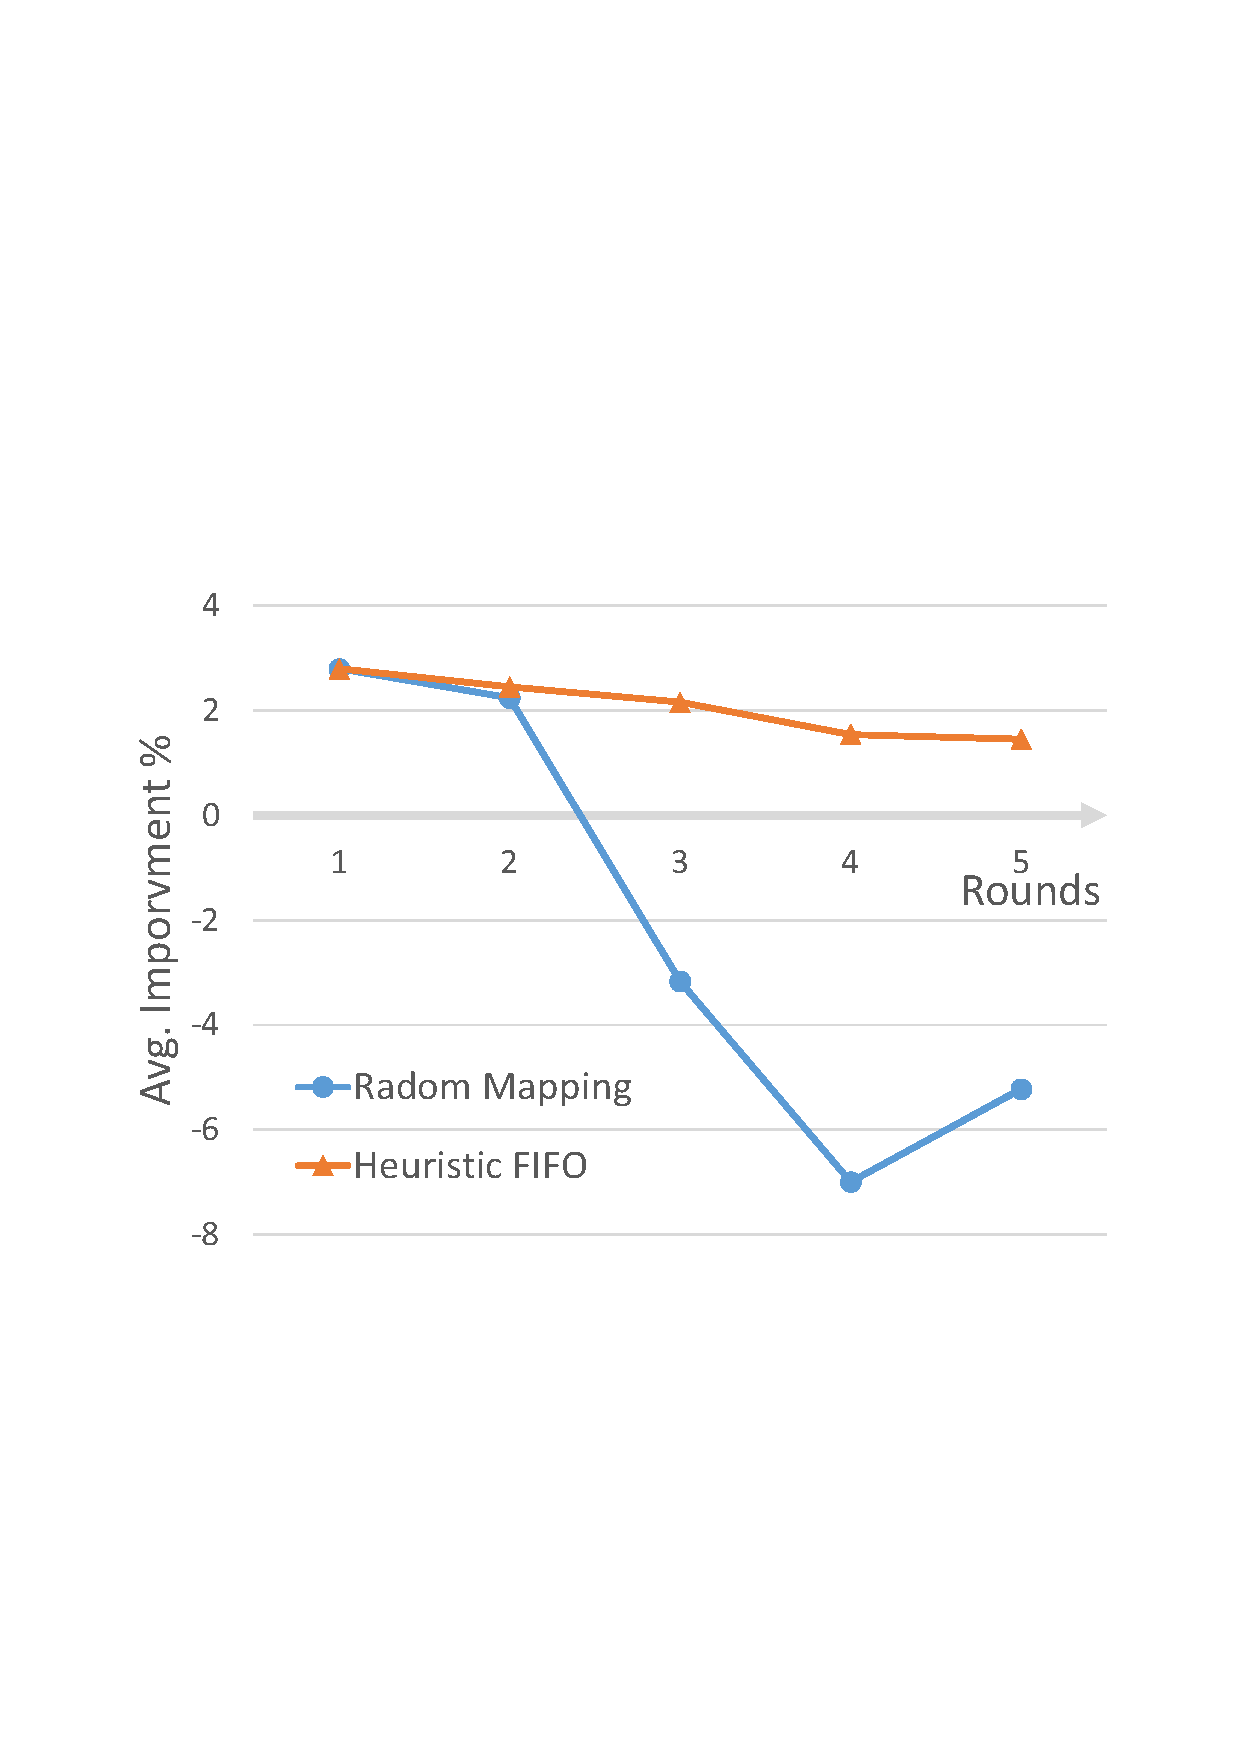
\includegraphics[width=\linewidth]{fig/sim}
				\caption{Stage Completion Time Improvement}
				\label{fig:sim}
			\end{subfigure}	
			\caption{Emulate Result of OpenCloud Trace}
		\end{figure}
	\end{minipage}
\end{figure*}
Note that since most of the traces from OpenCloud is shuffle-light workload as showen in Figure \ref{fig:cdf}. The average shuffle read time is 2.3\% of total reduce completion time. So we will only use this trace to evalute the pre-scheduling. 
\subsubsection{Random Task-Node Mapping}
The simplest way of pre-scheduling is mapping tasks to different nodes evenly. As shown in Figure \ref{fig:sim}, Random mapping works well when there is only one round of tasks in cluster. But multi-round in cluster is overwhleming according to Section \ref{multi}. The performance of random mapping collapses as the round number grows. After analyzing the trace, we find out that it's caused by data-skew. Reports in these papers\cite{skewtune, reining, gufler2012load} also claim that data-skew is commonly exist in data-parallel computing. When we apply a random mapping, it's probable to assign sevearl slow tasks on one node. The collision than slow down the the whole stage, which make the performance even worse than those without shuffle-prefetch. In addition, randomly assigned tasks also ignore the data locality between shuffle map output and shuffle reduce input, which can bring extra network traffic in cluster. 


\subsubsection{Shuffle Output Prediction}\label{shuffleprediction}
The failure of random mapping was obvious caused by application context (e.g. Shuffle input of each task) unawareness, which results in a heaver data skew. To avoid the 'bad' schedule results, we have to levrage the application context as assistance. The optimal schedule decision can be made under the awareness of shuffle dependecy number with input size for each task. unfortunately these data is unavialable when the pre-fetch starts. But the approximate size of each reduce task can be predicted using the prophase map output data with DAG context, so that the scheduling can approaching a more uniform load for each node.

According to the DAG computing process, the shuffle size of each reduce task is decided by input data, map task computation and hash partitioner. And for each map task, it will produce a data block for each reduce tasks, like '1-1' in Figure \ref{fig:shuffle}. '1-1' means it's produced by 'Map Task 1' for 'Reduce Task 1'. For Hadoop MapReduce, the shuffle input for each reduce task can be predicted with decent accuracy\cite{ishuffle}. They propose a liner regression model based on Verma et al.\cite{predict} that the ratio of map output size and input size is invariant given the same job configuration. Several map outputs (marked as Map Output in Figure \ref{fig:shuffle}) are picked as observation objects to train the model and than predict the final reduce distribution. But in the more sophisticated DAG computing framwork like Spark, this model can't fit. For instance, the reduce stage in Spark has more number of tasks that consume shuffle data instead of Hadoop MapReduce. More importantly, the customed partitioner can bring huge inconsistency between observed map output blocks distribution and the final reduce distribution, as we presented in Figure \ref{fig:dis}. We use different datasets with different partitioners to find the connection among three factors. We normalize threes sets of data to [0,1] to fit in one figure. In Figure \ref{fig:hash_pre}, we use a random input dataset with the Hash Partitioner of Spark\cite{sparksource}. In Figure \ref{fig:range_pre_sample}, we use a skew dataset with the Range Partitioner of Spark\cite{sparksource}.
We randomly pick one observation map output and plot. As we can see, in hash partitioner, the distribution of each map(blue area) is close to the final reduce distribution(orange boxes). The prediction results also turns out well fitted. As we apply linear regression model to predict the final reduce distribuiton of Range Partitioner. The prediction is severely effected by the skew observed map output distribution. 

To avoid this inconsistency in some cases, we introduce another methodology, weighted reservoir sampling, to mitigate this inconsistency. The classic reservoir samppling is designed for randomly chossing \textit{k} samples from \textit{n} items, where \textit{n} is either a very large or unknown number\cite{reservoir}. For each partition of data that produce shuffle output, we use reservoir sampling to randomly pick $s \times p$ of samples, where $p$ is the number of reduce tasks and $s$ is a tunable number. The number of input data partition and reduce tasks can be easily obtained when the from the DAG information. In Figure \ref{fig:range_pre_sample}, we set $s = 3$. Afther that, the map function is called locally to process the sampled data. As the 'Sampling' part showen in Figure \ref{fig:shuffle}, the final sampling map outputs are collected with the size of each parition of input data which is used as weight for each set of sample. For each reduce, the predicted size $reduceSize_i$

\begin{equation}
\label{equationsample} 
\begin{aligned}
	reduceSize_i = {\displaystyle\sum_{j=0}^{m} {partitionSize_j \times \frac{sample_i}{s \times p}}} \\ 
	{\left( m = \text{partition number of input data} \right)}
\end{aligned}
\end{equation}
As we can see in Figure \ref{fig:range_pre_sample}, the prediction result is much better even in a very skew scenario. The variance of the normalized data of sampling prediciton is because the strandard deviation of the prediction result is relatively small comparing to the average prediciton size, which is $0.0015$ in this example. Figure \ref{fig:prediction_relative_error} further prove that the sampling prediction can provide precise results even in the absoulte partition size of reduce tasks. On the oppsite, the result of linear regression comes out with huge relative error comparing with the fact of partition size of reduce tasks.
\begin{minipage}{\linewidth}
\begin{algorithm}[H]
\caption{Heuristic MinHeap Scheduling for Single Shuffle}
\label{hminheap}
	\begin{algorithmic}[1]
	\small
	\Procedure{schedule}{$m, h, p\_reduces$}
		\State $R\gets$ sort $p\_reduces$ by size
		\State $M\gets$ mapping of host id in $h$ to reduce id and size
		\State $rid\gets$ len$\left(R\right)$
		\Comment{Current scheduled reduce id}
		\While{$rid \geq 0$}
		\Comment{Schedule redues by MinHeap}
		\State Update $M\left[0\right].size$
		\State Assign $R\left(rid\right)$ to $M\left[0\right]$
		\State sift\_down$\left(M\left[0\right]\right)$
		\State
		\Comment{Use min-heap according to size in $M$}
		\State $rid\gets rid-1$
		\EndWhile
		\State $max\gets$ maximum size in $M$
		\State $rid\gets$ len$\left(R\right)$
		\While{$rid \geq 0$}
		\Comment{Heuristic swap by locality}
		\State $prob\gets$ max composition portion of $rid$
		\State $nor\gets \left(prob-1/m\right)/\left(1-1/m\right)/10$
		\State
		\Comment{Use $nor$ to limit the performance degradation in tasks swap}
		\State $t\_h\gets$ host that produces $prob$ data of $rid$
		\State $c\_h\gets$ current assigned host by MinHeap
		\If{$t\_h == c\_h$}
			\State Seal the assignment of $rid$ in $M$
		\Else
			\State swap\_tasks$\left(rid, c\_h, t\_h, max, nor\right)$
		\EndIf
		\State $rid\gets rid-1$
		\EndWhile
		% \Comment{$m$ is the number of input data}
		% \Comment{$r$ is partition number of reduces}
		% \Comment{$hosts$ is array of (hostid, partitionids[], size)}
		% \Comment{$c$ is $r*m$ array of composition data}
		% \Comment{$pSize$ is $r$ size array of predicted size of reduces}
		\Return $M$
	\EndProcedure
	\Procedure{swap\_tasks}{$rid, c\_h, t\_h, max, nor$}
	\State $num\gets$ number of reduces 
	\State selected from $t\_h$ that $total\_size$ won't
	\State make both $c\_h$ and $t\_h$ exceed $\left(1+nor\right)*max$
	\State after swapping
	\If{$num == 0$}
		\State return
	\Else
		\State \# Swap $nums$ of reduces with $rid$ between $c\_h$ and $t\_h$
		\State \# Update size of $t\_h$ and $c\_h$
	\EndIf
	\EndProcedure
	\end{algorithmic}
\end{algorithm}
\end{minipage}

But the sampling prediction may introduce a extral overhead in DAG computing process, we will evaluate the overhead in the Section \ref{evaluation}. Though in most cases, the overhead is negligible, but we won't use sampling for every reduce prediction. Combing with the DAG context, the sampling prediction will be triggered only when the range partitioner or customed partitioner occurs.

\subsubsection{Heuristic MinHeap Scheduling of Single Shuffle}\label{h-minheap}
For each predicted reduce size, a percentage array of total data composition among each map output is calculated. The highest percentage and it's corresponding host shoudle be the best choice the dimension of locality. In order to achieve the uniform load on each node while reducing the network traffic and shuffle transmission time. With this composition array and the predicted size of reduce, we present a heuristic MinHeap as the scheduling algorithm for single shuffle.

This algorithm can be divided into two round of scheduling. For input of $schedule$, $m$ is the partition number of input data, $h$ is the array of nodes ID in cluster and $p\_reduces$ is the predicted reduce matrix. Each row in $p\_reduces$ contains $r\_id$ as reduce partition ID, $size$ as predicted size of this partition, $prob$ as the maximum composition portion of reduce data, and $host$ as the node ID that produce the maximum portion of reduce data. As for $M$, it's a matrix consists $hostid$, $size$(total size of reduce data on this node) and an array of reduce id. 

In the first round (i.e. The first while in Alogorithm \ref{hminheap}), the reduces are first sorted by size. And then, they are assigned to hosts in the decending order of size . For hosts, we use a min-heap to maintain the hosts array according to the scheduled size on each hosts. In other word, the heavy tasks can be distributed evenly in the cluster.  After the scheduling, the completion time of reduce stage is close to the optimal. \textcolor{red}{may need to add math prove between this and optimal}. In the second round, the task-host mapping will be adjusted according to the locality. The closer $prob$ is to $1/m$, the more evenly this reduce is distributed in cluster. For a task which contains at most $prob$ data from $host$, the normalized probabilty $nor$ is calculated as a bound of performance degradation. This normalization can ensure that the more performance can be traded when the locality level increases. But the degradation of performance will not exceed 10\% since the maximum value of nor is 0.1 (in extream skew scenarios).  If the assigned host($c\_h$ in algorithm \ref{hminheap}) is not equal to the $host$ ($t\_h$ in algorithm \ref{hminheap}), than it has the $nor$ probality to trigger a tasks swap between two hosts. To maintain the scheduling mapping of first round, the tasks will only be swaped if the target hosts owns a set of tasks that has simmilar size totally. We use the OpenCloud\cite{opencloudtrace} trace to evaluate Heuristic MinHeap. Without swapping, the Heuristic MinHeap can acheieve a better performance improvement (average 5.7\%) than the default Spark FIFO scheduling algorithm (average 2.7\%). In the case of extream skew scenario, such as Figure \ref{fig:range_pre_sample}, Heuristic MinHeap trades about 0.05\% percent of stage completion time for 99\% reduction of shuffle data transmission through network by heruisticaly swapping tasks.

\begin{figure}
	\centering
	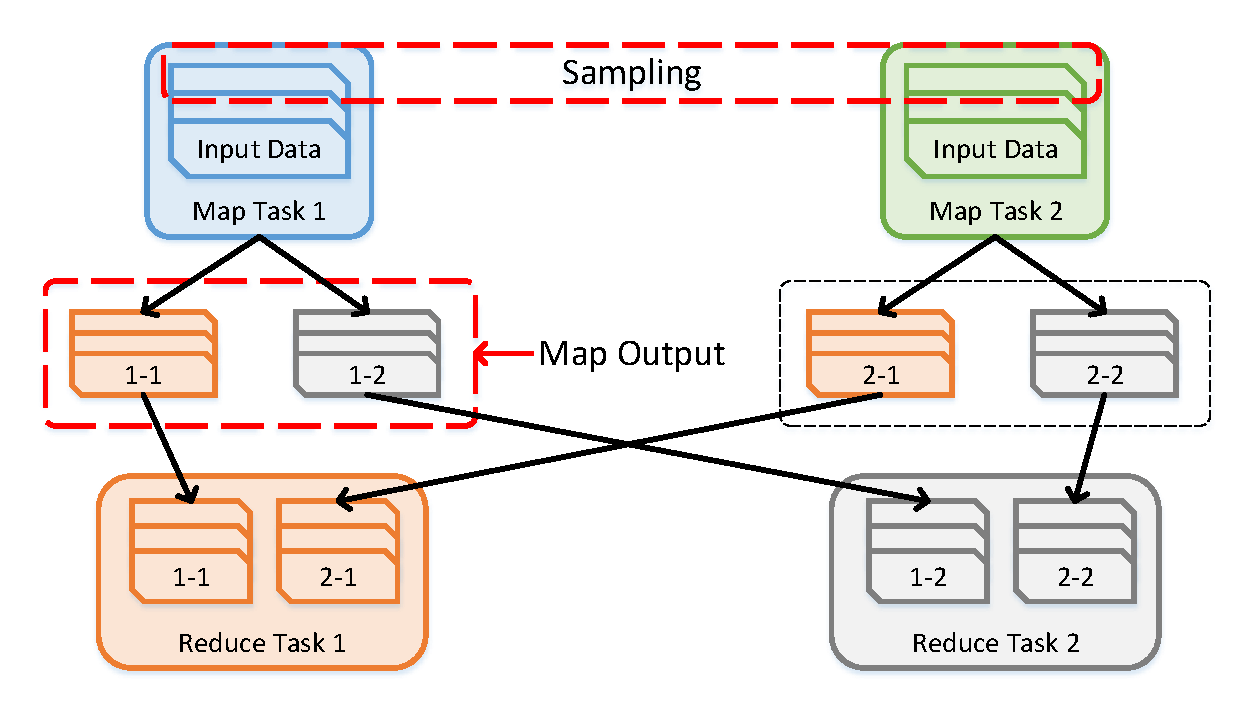
\includegraphics[width=\linewidth]{fig/shuffle}
	\caption{Shuffle Data Prediction}
	\label{fig:shuffle}
\end{figure}

\begin{figure*}
	\centering
	\begin{subfigure}[b]{0.32\linewidth}
		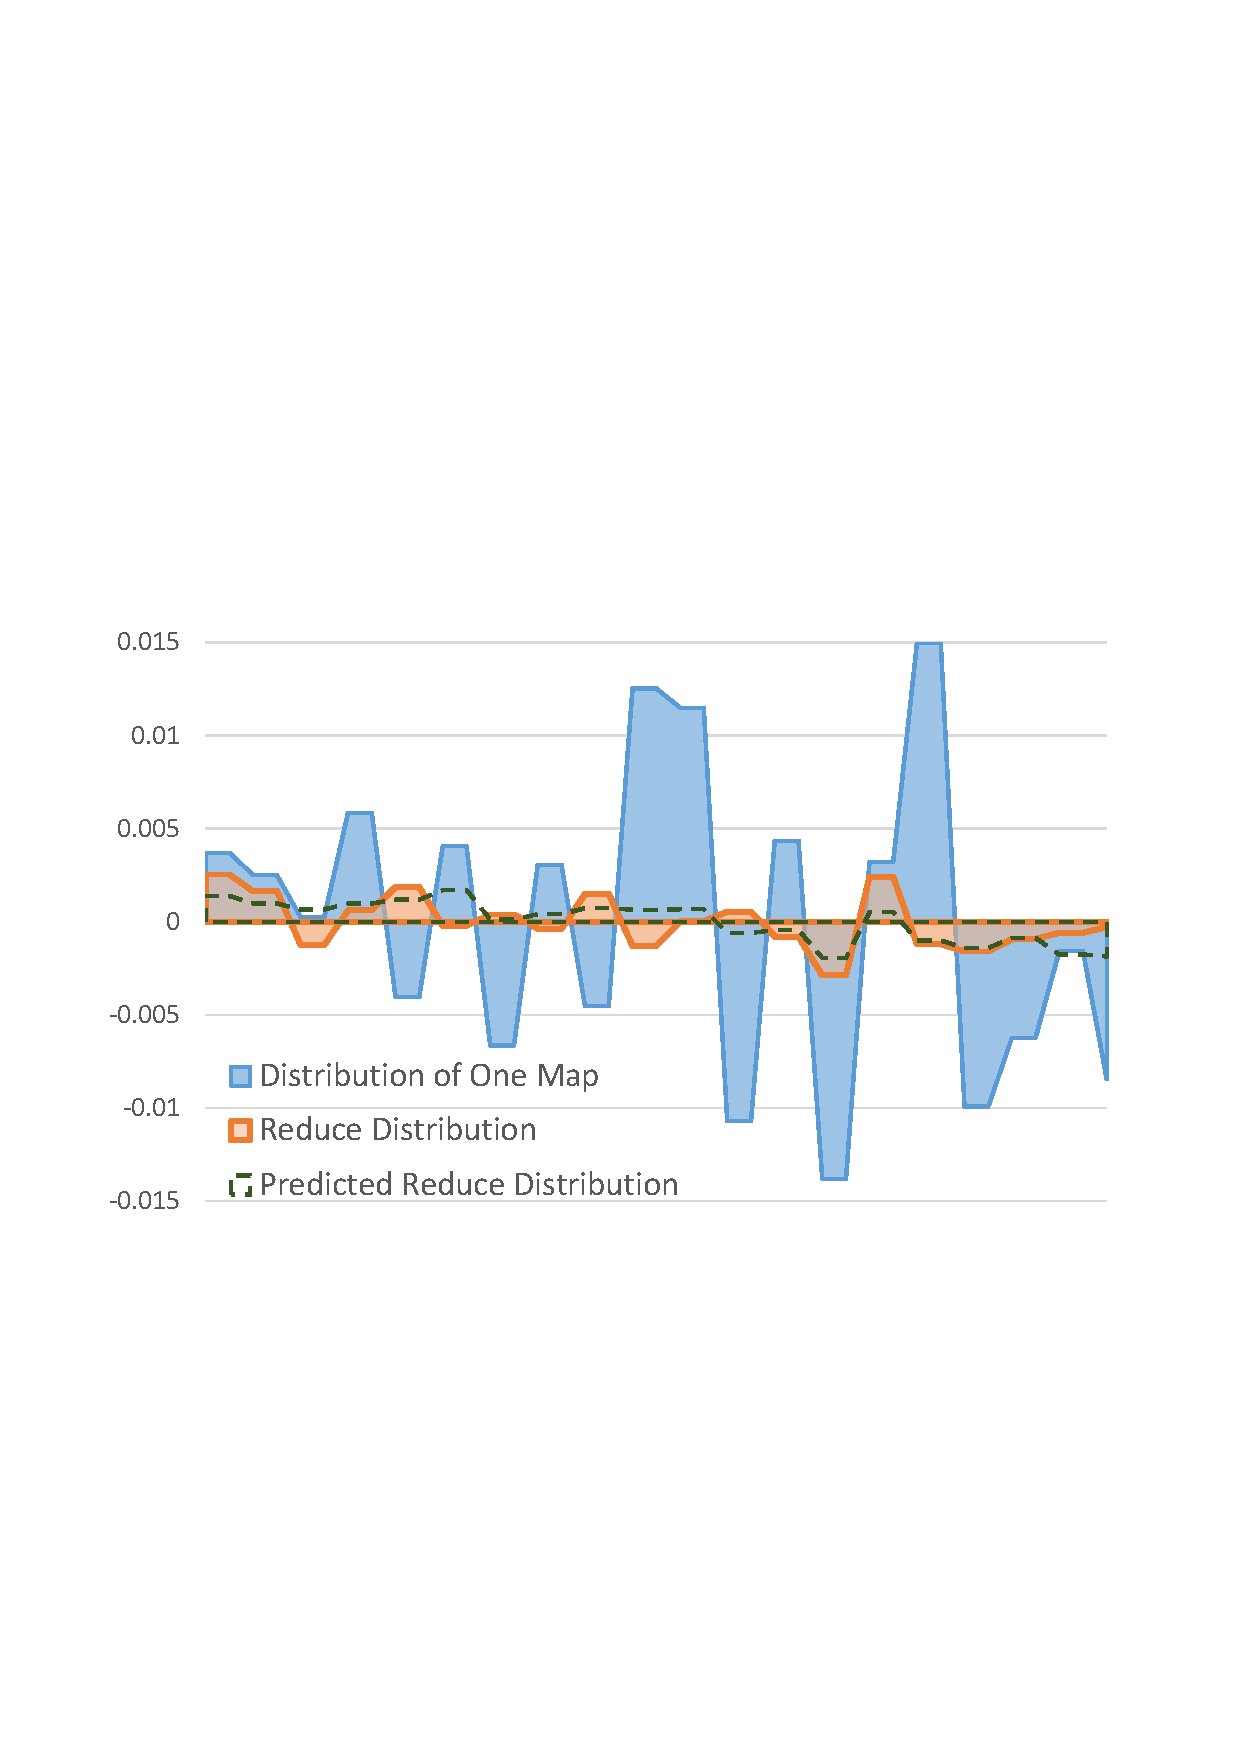
\includegraphics[width=\linewidth]{fig/hash_pre}
		\caption{Linear Regression Prediction of Hash Partitioner}
		\label{fig:hash_pre}
	\end{subfigure}
	\begin{subfigure}[b]{0.32\linewidth}
		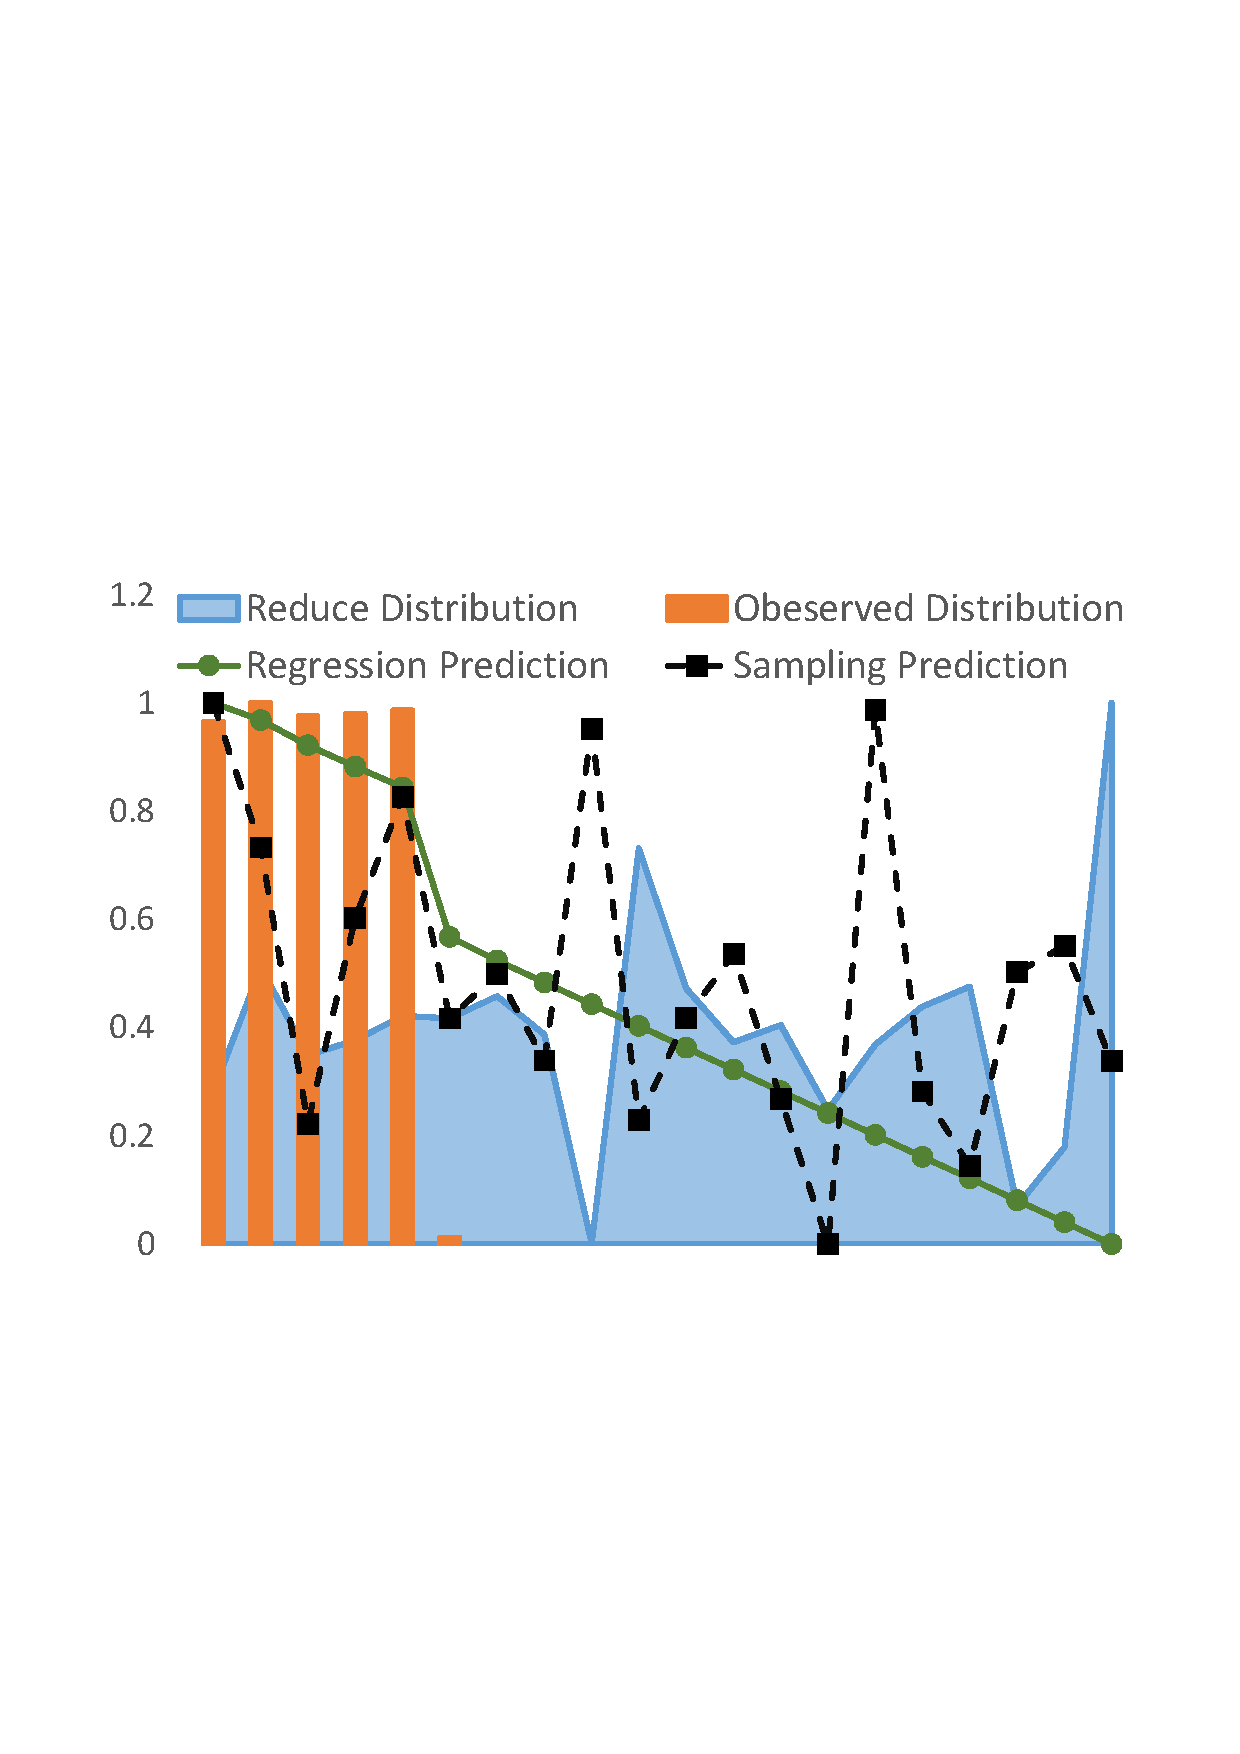
\includegraphics[width=\linewidth]{fig/range_pre_sample}
		\caption{Linear Regression and Sampling Prediction of Range Partitioner}
		\label{fig:range_pre_sample}
	\end{subfigure}
	\begin{subfigure}[b]{0.32\linewidth}
		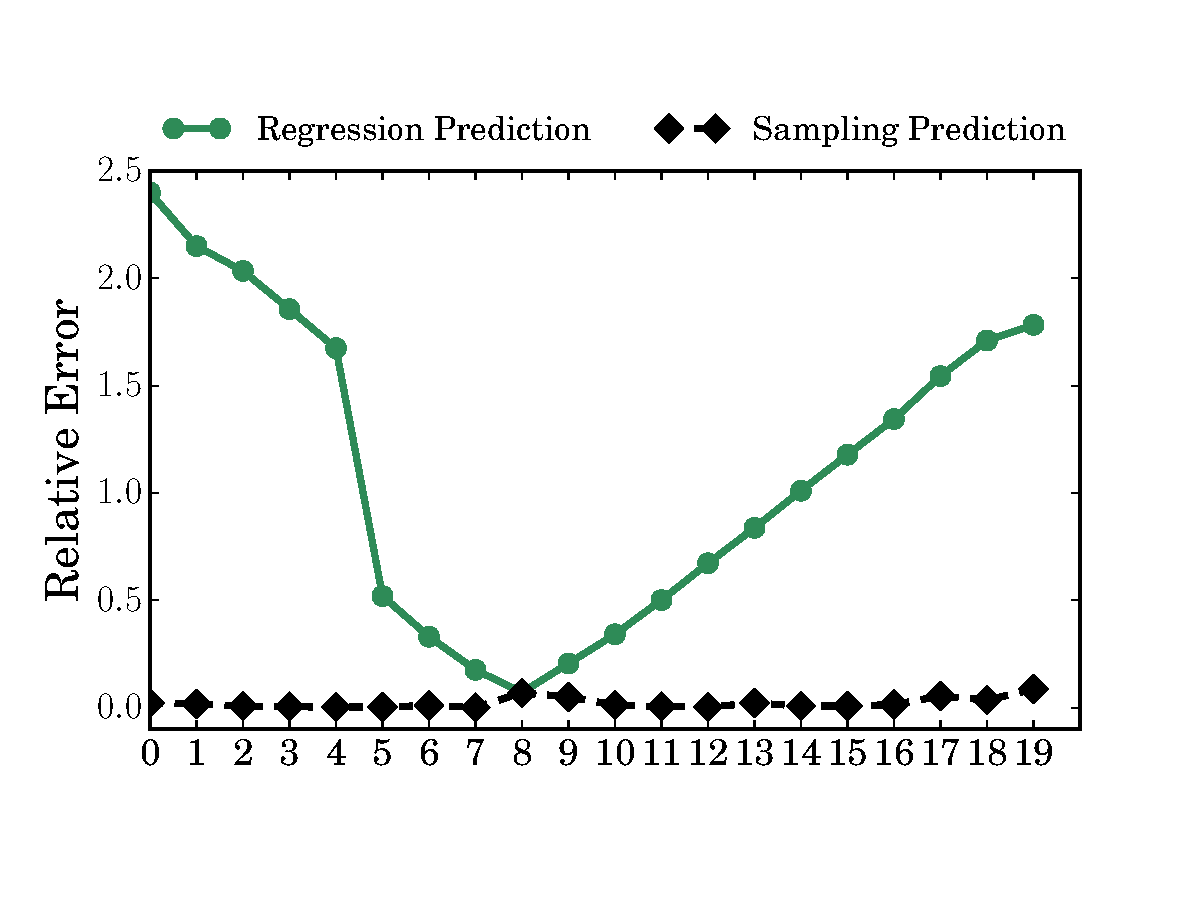
\includegraphics[width=\linewidth]{fig/prediction_relative_error}
		\caption{Prediction Relative Error of Range Partitioner}
		\label{fig:prediction_relative_error}
	\end{subfigure}
	\caption{Reduction Distribution Prediction}
	\label{fig:dis}
\end{figure*}
\subsubsection{Cope with Multiple Shuffles}
Unlike Hadoop MapReduce, multiple shuffles commonly exist in DAG computing. The techniques mention in Section \ref{shuffleprediction} can only predict the ongoing shuffle. For those pending shuffle, it's impossible to predict their size because of lacking either observed map outputs or sampling data. Let all tasks of all shuffle to be scheduled by DAG framework simultaneously can relieve the dilemma. But huge modification in DAG framework should be made by doing this. For example, Spark only supports one stage running at the same time for one application. To avoid this redundant workload, we provide the accumlating scheduling to cope with multiple shuffles.
\begin{minipage}{\linewidth}
\begin{algorithm}[H]
\caption{Accumulate Scheduling for Multi-Shuffles}
\label{mhminheap}
	\begin{algorithmic}[1]
	\small
	\Procedure{mSchedule}{$m, h, p\_reduces, shuffles$}
		\State
		\Comment $shuffles$ is the previous array of reduce partition ID, host ID and size
		\ForAll{$r\_id$ in $p\_reduces$}
		\State $p\_reduce\left[r\_id\right].size\gets p\_reduce\left[r\_id\right].size + shuffles\left[r\_id\right].size$
		\If{$shuffles\left[r\_id\right].size\geq p\_reduce\left[r\_id\right].size * p\_reduce\left[r\_id\right].prob$}
		\State Update $prob$ set $host$ to $shuffles\left[r\_id\right].host$
		\EndIf
		\EndFor
		\State $M\gets$ schedule$\left(m, h, p\_reduecs\right)$
		\ForAll{$host$ in $M$}
			\ForAll{$r\_id$ in $host$}
				\If{$host\neq shuffles\left[r\_id\right].host$}
				\State Re-shuffle data to $host$
				\State $shuffles\left[r\_id\right].host\gets host$
				\EndIf
			\EndFor
		\EndFor
		\Return $M$
	\EndProcedure
	\end{algorithmic}
\end{algorithm}
\end{minipage}

When a new shuffle start, the $mSchedule$ is called to schedule the current shuffle with previous $shuffles$. The size of reduce on each node of previous scheduled $shuffles$ are counted. Combined the with the predicted reduces size of current shuffle in $p\_reduces$, the $size$ of each reduce and its corresponding $porb$ and $host$ are updated accumulately. Then the $schedule$ is called to perform the shuffle scheduling. When the new host-reduce mapping is available, for each reduce task, if the new scheduled host in $M$ is not equle to the origin one, the re-shuffle will be triggered to transfer data to new scheduled host for further computing. This re-shuffle can be rare since the previous shuffled data in one reduce contributes a huge compostion while doing the accumulate updating. It means in the schedule phase, the $swap-task$ can help revise the scheduling to match the previous mapping in $shuffles$ as mucn as possible while maintaining the good performance.

\section{Implementation}\label{impl}
This section overviews the implementation of SCache -- a distributed in-memory storage system that caches shuffle data of DAG framework. Here we use Spark as example of DAG framwork to illustrate working process of shuffle optimization. We will first present system architecture in Subsection \ref{arch} while the following two subsections focuss on the two main challenges: memory manangement and fault tolerence.

\subsection{System Architecture}\label{arch}
SCache consists mainly two components: A distributed in-memory shuffle data storage system and the daemon inside Spark. As shown in Figure \ref{fig:arch}, for the in-memory storage system, SCache employs the legacy master-slaves architecture like GFS\cite{gfs}. The master node of SCache coordinates the shuffle blocks globally with application context from Spark. The coordination provides two guarantees: (a)store data in memory before tasks start and (b)schedule data on-off memory with all-or-nothing and strict priority constraints to benifit all jobs. 

When a Spark job starts, the DAG will be first generated by Spark DAGScheduler\cite{sparksource}. The process starts on the last result stage, and recursively find the dependent stages until the beginning of the DAG. While going forward to the beginning, the DAG computing pipeline will be cut off if a RDD in the stage has one or more shuffle dependencies. These shuffle dependencies among RDDs will then be submitted through RPC call to SCache master by a daemon process in Spark driver. For each shuffle dependency, the shuffle ID(an integer generated by Spark), the type of partitioner, the number of map tasks and the number of reduce tasks are included in the RPC call. The SCache master will store the metadata of one RPC call as a set of mutilpule shuffles scheduling unit. If there is a specialized partitioner, such as Range Partitioner or a customed paritioner, in the shuffle dependencies, the daemon will insert a sampling program in the host RDD that generates shuffle output using specialized partitioner. The sampling application will be scheduled ahead of that host RDD. We will illustrate the sampling procedure in the Section \ref{sampling}.

For the hash partitioner, when the map tasks in a stage finish computing on the work nodes, the  SCache Worker Daemon process will hijack the shuffle map output in the JVM of each executor of Spark (see Figure \ref{fig:arch}). Then the data will be transfered into the reserved memory of SCache Worker on each node through memory copy. In the same time, the Spark tasks will end after the memory copy without the disk shuffle output writing, which leads to a  reduction of the whole tasks completion time. When the shuffle map output block of a task is stored in the reserved memory, the SCache worker will then notify the master of the block belonging information with the reduce size distribution in this block (see Map Output in Figure \ref{fig:shuffle}). When the collected map output data reach the observed raito of map output, the SCache master will then run the scheduling algorithm \ref{mhminheap} (for multiple shuffle dependencies) and \ref{hminheap} (for single shuffle dependency) to get the reduce tasks -- nodes mapping. When the scheduling resulted is made, the master will then notify each worker to prepare the memory space for the shuffle data for reduce tasks. The pre-fetch of shuffle data as soon as each worker receives the scheduling results. More specifically, each worker will check the ID of reduce tasks that will be scheduled on itself in the future. When a map task finishs, each node will receive a broadcast message. It will then trigger the pre-fetch process to start fetching shuffle data from the memory of remote SCache worker that just finishs the map task. After all blocks of shuffle map output is transferred, the SCache worker will flush these blocks to disks for saving memory space and fault tolerence. 

Before the reduce stage starts, Spark DAG Scheduler will first generate a task set for this stage with different locality levels -- \textbf{\textit{PROCESS\_LOCAL, NODE\_LOCAL, NO\_PREF, RACK\_LOCAL, ANY}}. The locality levels are set by finding a cached location of a RDD. For the RDDs that have narrow dependency(oppsite ot shuffle dependency), the prefered location can also be the same as the depedent RDDs. For those RDDs that have shuffle dependecies, the locality will be set as \textbf{\textit{NO\_PREF}} by default. To enforce SCache pre-allocated the reduce tasks, we insert some lines of codes in Spark DAG Scheduler to consult SCache Master to get the preferred node for each tasks. By doing this, the tasks with shuffle dependencies can be set as \textbf{\textit{NODE\_LOCAL}}. Then the Task Scheduler will schedule tasks according to the task -- node mapping from SCache. 

When the scheduled reduce tasks start, the shuffle input data is requested. The SCache worker will then pass the requested data through memory copy from the reserved memory to Spark executor JVM memory. 

\subsubsection{Reservior Sampling}\label{sampling}
If the submitted shuffle dependencies contain a Rrange Partitioner or a customed partitioner, the SCache master will send a sampling request to the daemon process in Spark driver. The daemon process will then submit a job on Spark for the current RDD. This sampling job will use a reservoir sampling algorithm\cite{reservoir} on each partition of RDD since the items size of each partition is unknow before sampling. For the sample number, we set the size equals to $3 \times number\ of\ partitions$ for balancing overhead and accurancy (it can be tuned by configuration). The sampling job will then perform a local shuffle with the selected items and partitioner (see Figure \ref{fig:sample}). At the same time, the size of items is counted as the weight of each partition.These sampling data will be aggregated by $reduce\ ID$on SCache master. The size for each reduce partition can be easily computed by equation \ref{equationsample}. After the prediction, master will call algorithm \ref{mhminheap} and \ref{hminheap} to do the scheduling. 

\subsection{Memory Management}
As mentioned in section \ref{shufflesize}

\begin{figure}
	\centering
	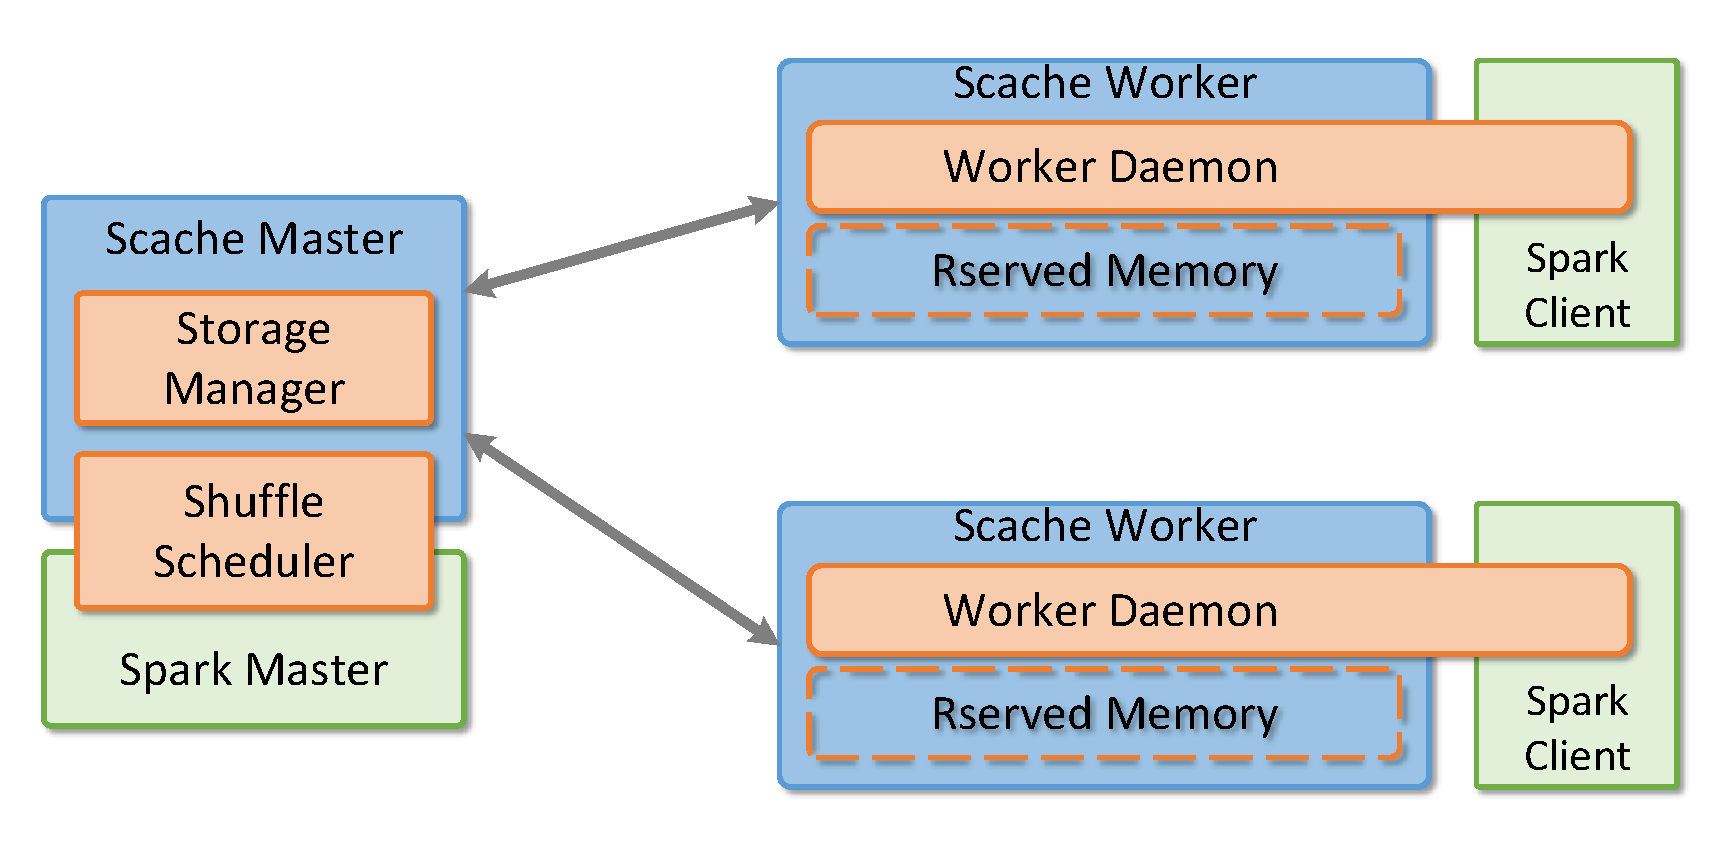
\includegraphics[width=\linewidth]{fig/arch}
	\caption{SCache Architecture}
	\label{fig:arch}
\end{figure}
\begin{figure}
	\centering
	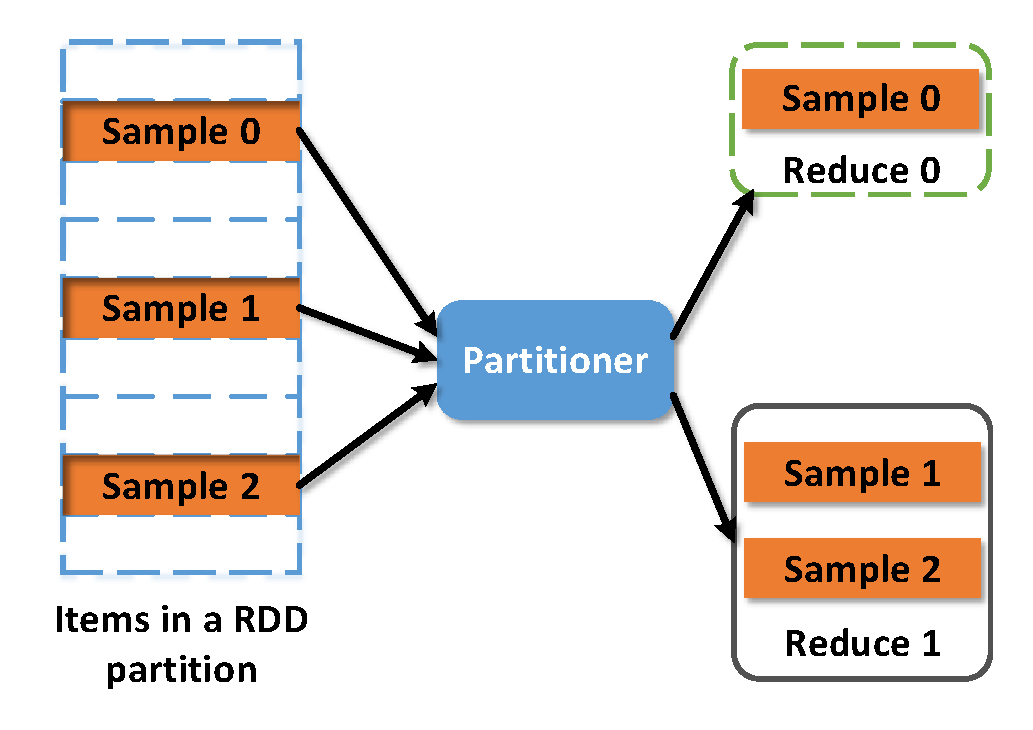
\includegraphics[width=\linewidth]{fig/sample}
	\caption{Demonstration of Reservoir Sampling}
	\label{fig:sample}
\end{figure}
\section{Evaluation}\label{evaluation}

\section{Conclusion}



\bibliographystyle{abbrv}
\bibliography{biblio}

\end{document}


